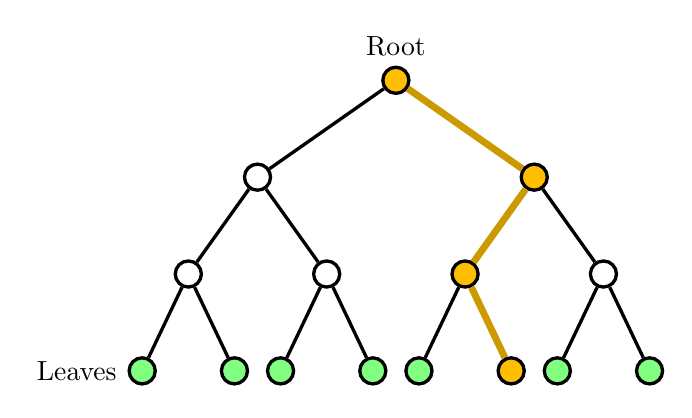
\begin{tikzpicture}[
  level/.style={
    sibling distance = 10.0em/#1,
    level distance = 3.5em
  },
  node/.style={
    draw,
    circle,
    very thick,
    color=black,
    fill=white
  },
  node_filled/.style={
    node,
    color=black,
    fill=orange!50!yellow
  },
  node_leaf/.style={
    node,
    color=black,
    fill=green!50!white,
  },
  path/.style={
    draw,
    line width=0.25em,
    color=orange!50!yellow!80!black
  },
  path_normal/.style={
    draw,
    very thick,
    color=black
  }
]%
\node [node_filled, label={[anchor=south]above:Root}] (root) {}
child [path_normal] {
  node [node] {}
  child {
    node [node] {}
    child {node [node_leaf, label={[anchor=east]left:Leaves}] {}}
    child {node [node_leaf] {}}
  }
  child {
    node [node] {}
    child {node [node_leaf] {}}
    child {node [node_leaf] {}}
  }
}
child [path] {
  node [node_filled] {}
  child {
    node [node_filled] {}
    child [path_normal] {node [node_leaf] {}}
    child {node [node_filled] {}}
  }
  child [path_normal] {
    node [node] {}
    child {node [node_leaf] {}}
    child {node [node_leaf] {}}
  }
};
\end{tikzpicture}